\documentclass[tikz,border=10pt]{standalone}
\usepackage{helvet}
\renewcommand{\familydefault}{\sfdefault}
\usepackage{amsmath}
\usepackage{tikz}
\usetikzlibrary{positioning, calc, arrows.meta, shapes.geometric, decorations.pathreplacing, fit}

\definecolor{emeraldpine}{HTML}{1A4D3E}
\definecolor{harvardcrimson}{HTML}{A51C30}
\definecolor{ethdarkblue}{HTML}{1F407A}
\definecolor{ethpetrol}{HTML}{007A87}
\definecolor{ethbronze}{HTML}{B87333}
\definecolor{ink}{HTML}{1A202C}
\definecolor{softink}{HTML}{4A5568}
\definecolor{cardbg}{HTML}{F8FAFC}

\begin{document}
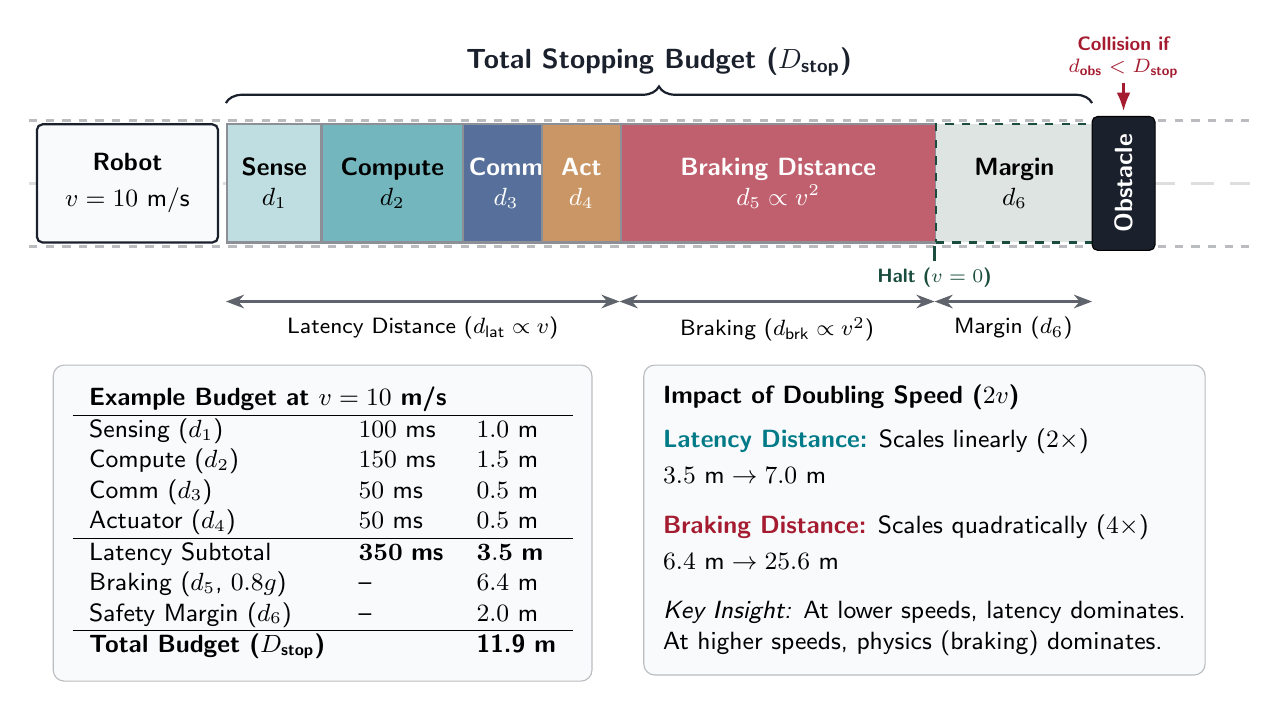
\begin{tikzpicture}[
    font=\sffamily\small,
    >={Stealth[length=5pt,width=4pt]},
    robot/.style={draw=ink, fill=cardbg, thick, minimum width=2.3cm, minimum height=1.5cm, rounded corners=2pt, align=center},
    zone/.style={draw=ink!50, thick, minimum height=1.5cm, align=center, inner sep=2pt},
    dim/.style={draw=ink!70, <->, >=Stealth, thick},
    brace/.style={decorate, decoration={brace, amplitude=6pt, raise=2pt}, thick, ink}
]

    % Grid/Road
    \draw[dashed, ink!30, line width=1pt] (0, 0) -- (15.5, 0);
    \draw[dashed, ink!30, line width=1pt] (0, -1.6) -- (15.5, -1.6);

    % Road Centerline
    \draw[dash pattern=on 8pt off 6pt, ink!15, line width=0.8pt] (0, -0.8) -- (15.5, -0.8);

    % Robot
    \def\zY{-0.8}
    \node[robot] (robo) at (1.25, \zY) {\textbf{Robot}\\[2pt]$v = 10\text{ m/s}$};
    
    % Start point x = 2.5 (front of robot)
    % Zone 1: Sense (1.2cm)
    \node[zone, fill=ethpetrol!25, minimum width=1.2cm, anchor=west] (z1) at (2.5, \zY) {\textbf{Sense}\\$d_1$};
    % Zone 2: Compute (1.8cm)
    \node[zone, fill=ethpetrol!55, minimum width=1.8cm, anchor=west] (z2) at (3.7, \zY) {\textbf{Compute}\\$d_2$};
    % Zone 3: Comm (1.0cm)
    \node[zone, fill=ethdarkblue!75, text=white, minimum width=1.0cm, anchor=west] (z3) at (5.5, \zY) {\textbf{Comm}\\$d_3$};
    % Zone 4: Actuator (1.0cm)
    \node[zone, fill=ethbronze!75, text=white, minimum width=1.0cm, anchor=west] (z4) at (6.5, \zY) {\textbf{Act}\\$d_4$};
    % Zone 5: Braking (4.0cm)
    \node[zone, fill=harvardcrimson!70, text=white, minimum width=4.0cm, anchor=west] (z5) at (7.5, \zY) {\textbf{Braking Distance}\\$d_5 \propto v^2$};
    % Zone 6: Margin (2.0cm)
    \node[zone, draw=emeraldpine, dashed, fill=emeraldpine!15, minimum width=2.0cm, anchor=west] (z6) at (11.5, \zY) {\textbf{Margin}\\$d_6$};

    % Vehicle Halt Marker
    \draw[emeraldpine, line width=1.2pt] (11.5, -1.6) -- (11.5, -1.78);
    \node[font=\scriptsize\bfseries, text=emeraldpine, anchor=north] at (11.5, -1.75) {Halt ($v=0$)};

    % Obstacle (placed at the boundary of the stopping budget)
    \draw[fill=ink, rounded corners=2pt] (13.5, 0.05) rectangle (14.3, -1.65) node[pos=0.5, text=white, rotate=90, font=\bfseries\small] {Obstacle};

    % Total Distance Brace
    \draw[brace] (2.5, 0.15) -- (13.5, 0.15) node[midway, above=8pt, font=\bfseries] {Total Stopping Budget ($D_{\text{stop}}$)};

    % Obstacle & Hazard Callout
    \node[font=\scriptsize\bfseries, text=harvardcrimson, align=center] at (13.9, 0.8) {Collision if\\$d_{\text{obs}} < D_{\text{stop}}$};
    \draw[-Latex, harvardcrimson, thick] (13.9, 0.48) -- (13.9, 0.12);

    % Distance Dimension Annotations
    \draw[dim] (2.5, -2.3) -- (7.5, -2.3) node[midway, below=2pt, font=\footnotesize] {Latency Distance ($d_{\text{lat}} \propto v$)};
    \draw[dim] (7.5, -2.3) -- (11.5, -2.3) node[midway, below=2pt, font=\footnotesize] {Braking ($d_{\text{brk}} \propto v^2$)};
    \draw[dim] (11.5, -2.3) -- (13.5, -2.3) node[midway, below=2pt, font=\footnotesize] {Margin ($d_6$)};
    
    % Table for example numbers
    \node[anchor=north west, draw=ink!30, rounded corners=4pt, fill=cardbg, inner sep=7pt] at (0.3, -3.1) {
        \begin{tabular}{l l l}
        \multicolumn{3}{l}{\textbf{Example Budget at $v = 10$ m/s}} \\
        \hline
        Sensing ($d_1$)   & $100$ ms & $1.0$ m \\
        Compute ($d_2$)   & $150$ ms & $1.5$ m \\
        Comm ($d_3$)      & $50$ ms  & $0.5$ m \\
        Actuator ($d_4$)  & $50$ ms  & $0.5$ m \\
        \hline
        Latency Subtotal  & $\mathbf{350}$ \textbf{ms} & $\mathbf{3.5}$ \textbf{m} \\
        Braking ($d_5$, $0.8g$) & -- & $6.4$ m \\
        Safety Margin ($d_6$)   & -- & $2.0$ m \\
        \hline
        \textbf{Total Budget ($D_{\text{stop}}$)} & & \textbf{11.9 m}
        \end{tabular}
    };

    % Speed Scaling Comparison
    \node[anchor=north west, draw=ink!30, rounded corners=4pt, fill=cardbg, inner sep=7pt, align=left] at (7.8, -3.1) {
        \textbf{Impact of Doubling Speed ($2v$)}\\[5pt]
        \textcolor{ethpetrol}{\textbf{Latency Distance:}} Scales linearly ($2\times$)\\[2pt]
        $3.5\text{ m} \rightarrow 7.0\text{ m}$\\[7pt]
        \textcolor{harvardcrimson}{\textbf{Braking Distance:}} Scales quadratically ($4\times$)\\[2pt]
        $6.4\text{ m} \rightarrow 25.6\text{ m}$\\[7pt]
        \textit{Key Insight:} At lower speeds, latency dominates.\\
        At higher speeds, physics (braking) dominates.
    };

\end{tikzpicture}
\end{document}
